\clearpage

\subsection{Transparent with 1+1 Protection}\label{heuristic_Transp_Protection}
\begin{tcolorbox}	
\begin{tabular}{p{2.75cm} p{0.2cm} p{10.5cm}} 	
\textbf{Student Name}  &:& Pedro Coelho    (March 01, 2018 - )\\
\textbf{Goal}          &:& Implement the heuristic model for the transparent transport mode with 1 plus 1 protection.
\end{tabular}
\end{tcolorbox}

\subsubsection{Model description}

\vspace{11pt}
Contrary to the transparent without survivability transport mode, the transparent with 1+1 protection technique has a backup path, so if there is a network failure it is more likely to not suffer large data losses. The backup paths are always different from the primary ones and they prevent that the information going through optical channels could be lost in these occasions. However, the CAPEX will be significantly higher (more than the double), because that includes a secondary path that will increase several network elements.

After the creation of the matrices and the network topology, it is necessary to apply the routing and grooming algorithms created. In the end, a report algorithm will be applied to obtain the best CAPEX result for the network in question.

We also must take into account the following particularity of this mode of transport:
\begin{itemize}
  \item $N_{OXC,n}$ = 1, \quad $\forall$ n that process traffic
  \item $N_{EXC,n}$ = 1, \quad $\forall$ n that process traffic
\end{itemize}

\vspace{11pt}
The minimization of the network CAPEX is made through the equation \ref{Capex_heuristic} where in this case for the cost of nodes we have in consideration the electric cost \ref{Capex_Node_EXC_heuristic} and the optical cost \ref{Capex_Node_OXC_heuristic}.
In this case the value of $P_{exc,c,n}$ is obtained by equation \ref{EXC_pexc_transparentp_heuristic_protec} and the value of $P_{oxc,n}$ is obtained by equation \ref{OXC_poxc_transparentp_heuristic_protec}.\\

The equation \ref{EXC_pexc_transparentp_heuristic_protec} refers to the number of short-reach ports of the electrical switch with bit-rate $c$ in node $n$, $P_{exc,c,n}$, i.e. the number of tributary ports with bit-rate $c$ in node $n$ which can be calculated as

\begin{equation}
P_{exc,c,n} = 2 \sum_{d=1}^{N} D_{nd,c}
\label{EXC_pexc_transparentp_heuristic_protec}
\end{equation}

\vspace{11pt}
where $D_{nd,c}$ are the client demands between nodes $n$ and $d$ with bit rate $c$.

\vspace{11pt}
In this case there is the following particularity:

\begin{itemize}
  \item When $n$=$d$ the value of client demands is always zero, i.e, $D_{nn,c}=0$
\end{itemize}

\vspace{11pt}
The equation \ref{OXC_poxc_transparentp_heuristic_protec} refers to the number of long-reach ports of the optical switch in node $n$, $P_{oxc,n}$, i.e. the number of line ports and the number of adding ports of node $n$ which can be calculated as

\begin{equation}
P_{oxc,n} = \sum_{j=1}^{N} f_{nj} + \sum_{j=1}^{N} \lambda_{nj}
\label{OXC_poxc_transparentp_heuristic_protec}
\end{equation}

\vspace{11pt}
where $f_{nj}$ refers to the number of line ports and $\lambda_{nj}$ refers to the number of adding ports.

\vspace{17pt}
The function, to be minimized, is the expression \ref{Minimize_Heuristic_CAPEX}.\\

\subsubsection{Result description}

It is already known all the necessary formulas to obtain the CAPEX value for the reference network \ref{Reference_Network_Topology}. As described in the subsection of the network traffic \ref{Reference_Network_Traffic}, it is necessary to obtain three different values of CAPEX for the low (0.5 Tbit/s), medium (5 Tbit/s) and high (10 Tbit/s) traffic. It is used a network software program called Net2Plan which can design the traffic matrices, create all the network topologies, simulate the algorithms into the network implemented in the programming software called Eclipse and analyze the results obtained.

In this chapter will be demonstrated the results by Vasco's heuristics from 2016. In each of the three traffic scenarios, it will be shown the network topologies followed by the table with the CAPEX value of the network.\\

\textbf{Low Traffic Scenario:}\\

In this scenario we have to take into account the traffic calculated in \ref{low_scenario}. In a first phase we will show the various existing topologies of the network. The first are the allowed topologies, physical and optical topology, the second are the logical topology for all ODUs and finally the resulting physical and optical topology.\\

\begin{figure}[H]
\centering
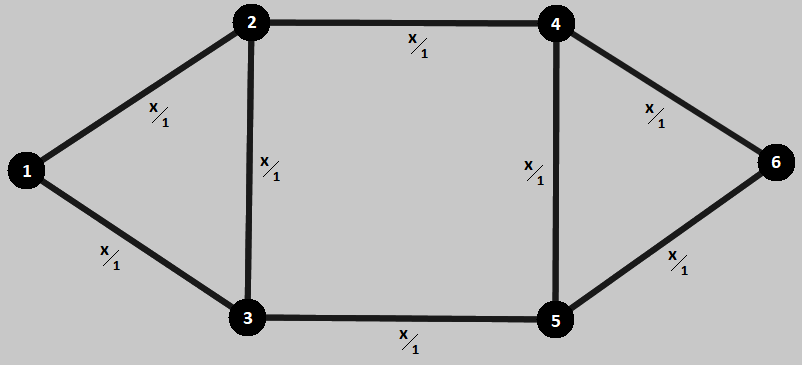
\includegraphics[width=13cm]{sdf/heuristic/transparent_protection/low/allowed_physical_low}
\caption{Allowed physical topology. The allowed physical topology is defined by the duct and sites in the field. It is assumed that each duct supports up to 1 bidirectional transmission system and each site supports up to 1 node.}
\label{allowed_physical_protection_ref_low_heuristic_transparent}
\end{figure}

\begin{figure}[H]
\centering
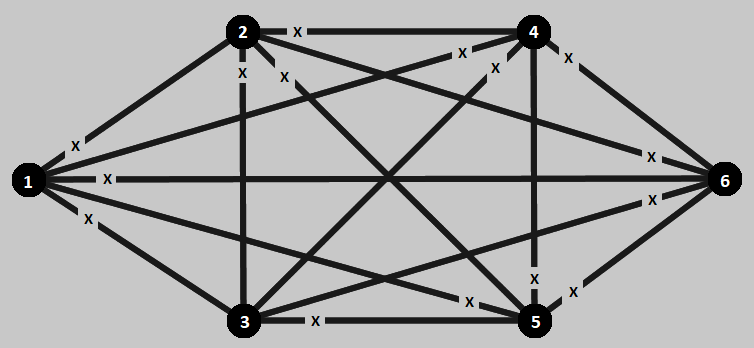
\includegraphics[width=13cm]{sdf/heuristic/transparent_protection/low/allowed_optical_low}
\caption{Allowed optical topology. The allowed optical topology is defined by the transport mode (transparent transport mode in this case). It is assumed that each connections between demands supports up to 100 lightpaths.}
\label{allowed_optical_protection_ref_low_heuristic_transparent}
\end{figure}

\begin{figure}[H]
\centering
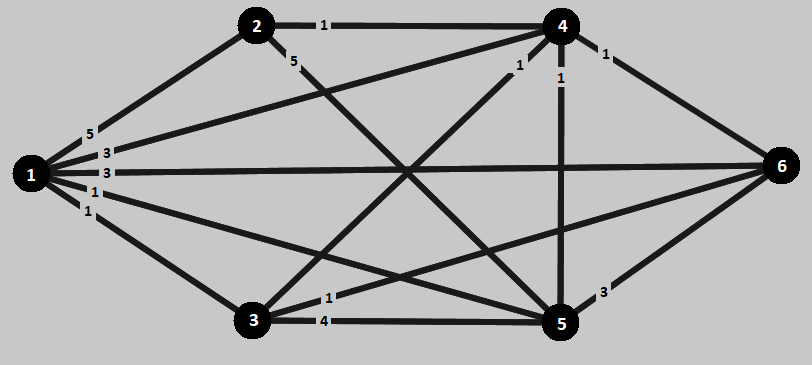
\includegraphics[width=13cm]{sdf/heuristic/transparent_protection/low/logical_topology_odu0_low}
\caption{ODU0 logical topology defined by the ODU0 traffic matrix.}
\label{logical_ODU0_protection_ref_low_heuristic_transparent}
\end{figure}

\begin{figure}[H]
\centering
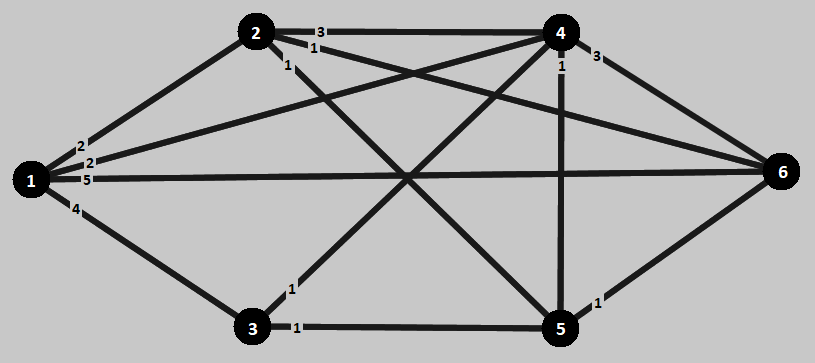
\includegraphics[width=13cm]{sdf/heuristic/transparent_protection/low/logical_topology_odu1_low}
\caption{ODU1 logical topology defined by the ODU1 traffic matrix.}
\label{logical_ODU1_protection_ref_low_heuristic_transparent}
\end{figure}

\begin{figure}[H]
\centering
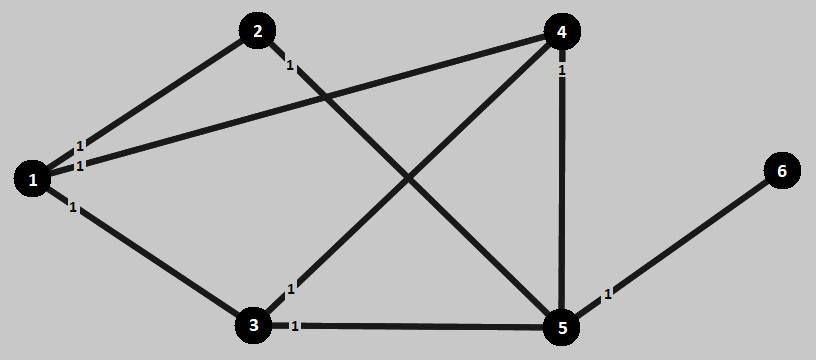
\includegraphics[width=13cm]{sdf/heuristic/transparent_protection/low/logical_topology_odu2_low}
\caption{ODU2 logical topology defined by the ODU2 traffic matrix.}
\label{logical_ODU2_protection_ref_low_heuristic_transparent}
\end{figure}

\begin{figure}[H]
\centering
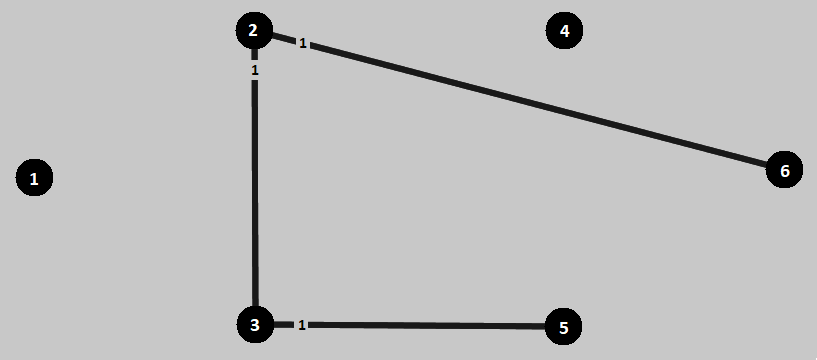
\includegraphics[width=13cm]{sdf/heuristic/transparent_protection/low/logical_topology_odu3_low}
\caption{ODU3 logical topology defined by the ODU3 traffic matrix.}
\label{logical_ODU3_protection_ref_low_heuristic_transparent}
\end{figure}

\begin{figure}[H]
\centering
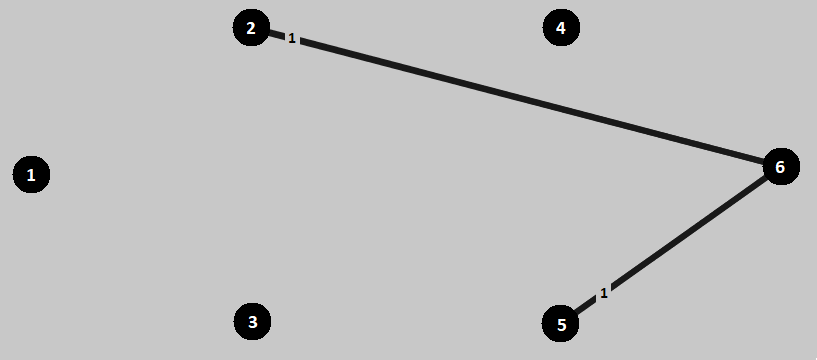
\includegraphics[width=13cm]{sdf/heuristic/transparent_protection/low/logical_topology_odu4_low}
\caption{ODU4 logical topology defined by the ODU4 traffic matrix.}
\label{logical_ODU4_protection_ref_low_heuristic_transparent}
\end{figure}

\begin{figure}[H]
\centering
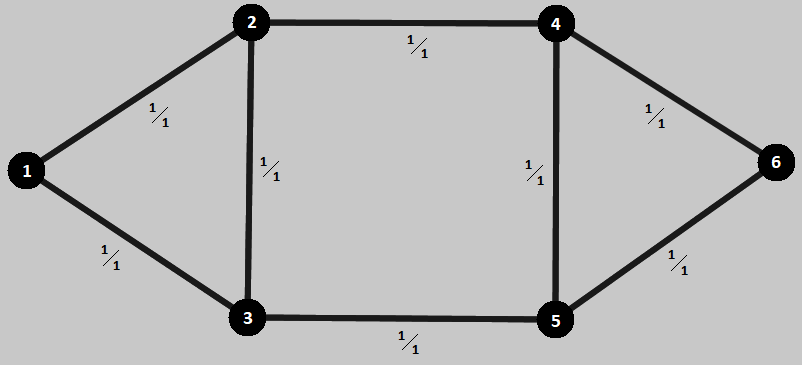
\includegraphics[width=13cm]{sdf/heuristic/transparent_protection/low/physical_topology_low}
\caption{Physical topology after dimensioning.}
\label{physical_topology_protection_ref_low_heuristic_transparent}
\end{figure}

Following all the steps mentioned in the \ref{net2plan_guide}, applying the routing and grooming heuristic algorithms in the Net2Plan software and using all the data referring to this scenario, the obtained result for the Vasco's heuristics can be consulted in the following table \ref{scripttransp_protec_ref_low_heuristic}.

\begin{table}[H]
\centering
\begin{tabular}{|| c | c | c | c | c | c | c ||}
 \hline
 \multicolumn{7}{|| c ||}{CAPEX of the Network} \\
 \hline
 \hline
 \multicolumn{3}{|| c |}{ } & Quantity & Unit Price & Cost & Total \\
 \hline
 \multirow{3}{*}{Link Cost} & \multicolumn{2}{ c |}{OLTs} & 16 & 15 000 \euro & 240 000 \euro & \multirow{3}{*}{68 520 000 \euro} \\ \cline{2-6}
 & \multicolumn{2}{ c |}{100 Gb/s Transceivers} & 136 & 5 000 \euro/Gb/s & 68 000 000 \euro & \\ \cline{2-6}
 & \multicolumn{2}{ c |}{Amplifiers} & 70 & 4 000 \euro & 280 000 \euro & \\
 \hline
 \multirow{10}{*}{Node Cost} & \multirow{7}{*}{Electrical} & EXCs & 6 & 10 000 \euro & 60 000 \euro & \multirow{10}{*}{14 547 590 \euro} \\ \cline{3-6}
  & & ODU0 Ports & 60 & 10 \euro & 600 \euro & \\ \cline{3-6}
 & & ODU1 Ports & 50 & 15 \euro & 750 \euro & \\ \cline{3-6}
 & & ODU2 Ports & 16 & 30 \euro & 480 \euro & \\ \cline{3-6}
 & & ODU3 Ports & 6 & 60 \euro & 360 \euro & \\ \cline{3-6}
 & & ODU4 Ports & 4 & 100 \euro & 400 \euro & \\ \cline{3-6}
 & & Line Ports & 136 & 1 000 \euro/Gb/s & 13 600 000 \euro & \\ \cline{3-6}
 & \multirow{3}{*}{Optical} & OXCs & 6 & 20 000 \euro & 120 000 \euro & \\ \cline{3-6}
 & & Line Ports & 272 & 2 500 \euro/porto & 680 000 \euro & \\ \cline{3-6}
 & & Add Ports & 34 & 2 500 \euro/porto & 85 000 \euro & \\
 \hline
 \multicolumn{6}{|| c |}{Total Network Cost} & 83 067 590 \euro \\
\hline
\end{tabular}
\caption{Table with detailed description of CAPEX of Vasco's 2016 results.}
\label{scripttransp_protec_ref_low_heuristic}
\end{table}

\textbf{Medium Traffic Scenario:}\\

In this scenario we have to take into account the traffic calculated in \ref{medium_traffic_scenario}. In a first phase we will show the various existing topologies of the network. The first are the allowed topologies, physical and optical topology, the second are the logical topology for all ODUs and finally the resulting physical and optical topology.\\

\begin{figure}[H]
\centering
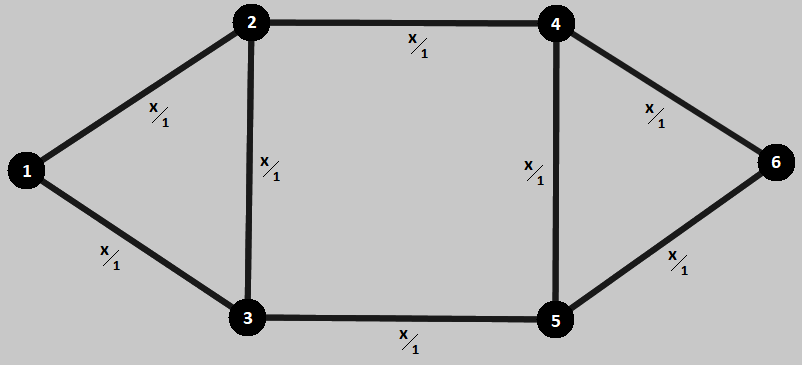
\includegraphics[width=13cm]{sdf/heuristic/transparent_protection/medium/allowed_physical_medium}
\caption{Allowed physical topology. The allowed physical topology is defined by the duct and sites in the field. It is assumed that each duct supports up to 1 bidirectional transmission system and each site supports up to 1 node.}
\label{allowed_physical_protection_ref_medium_heuristic_transparent}
\end{figure}

\begin{figure}[H]
\centering
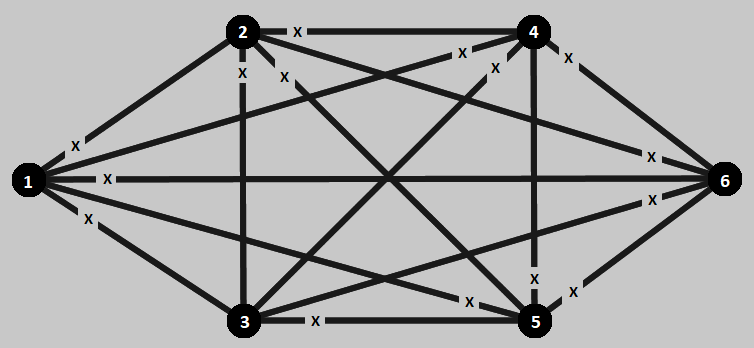
\includegraphics[width=13cm]{sdf/heuristic/transparent_protection/medium/allowed_optical_medium}
\caption{Allowed optical topology. The allowed optical topology is defined by the transport mode (transparent transport mode in this case). It is assumed that each connections between demands supports up to 100 lightpaths.}
\label{allowed_optical_protection_ref_medium_heuristic_transparent}
\end{figure}

\begin{figure}[H]
\centering
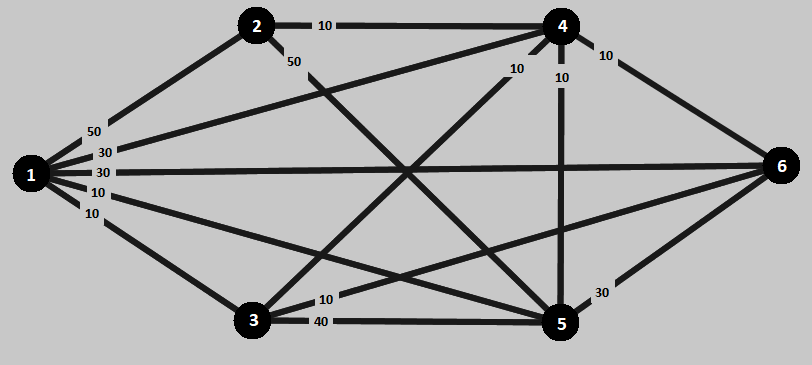
\includegraphics[width=13cm]{sdf/heuristic/transparent_protection/medium/logical_topology_odu0_medium}
\caption{ODU0 logical topology defined by the ODU0 traffic matrix.}
\label{logical_ODU0_protection_ref_medium_heuristic_transparent}
\end{figure}

\begin{figure}[H]
\centering
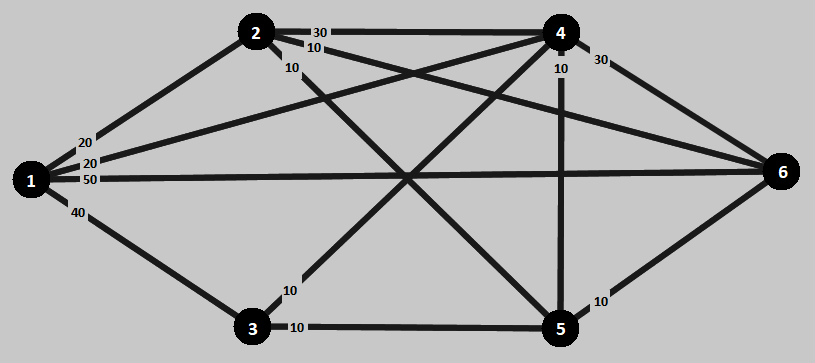
\includegraphics[width=13cm]{sdf/heuristic/transparent_protection/medium/logical_topology_odu1_medium}
\caption{ODU1 logical topology defined by the ODU1 traffic matrix.}
\label{logical_ODU1_protection_ref_medium_heuristic_transparent}
\end{figure}

\begin{figure}[H]
\centering
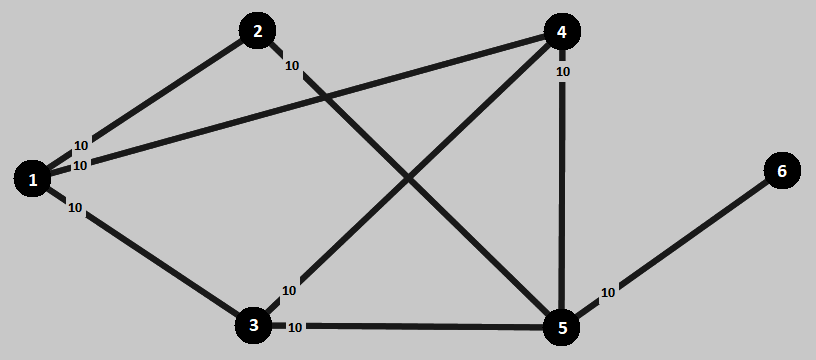
\includegraphics[width=13cm]{sdf/heuristic/transparent_protection/medium/logical_topology_odu2_medium}
\caption{ODU2 logical topology defined by the ODU2 traffic matrix.}
\label{logical_ODU2_protection_ref_medium_heuristic_transparent}
\end{figure}

\begin{figure}[H]
\centering
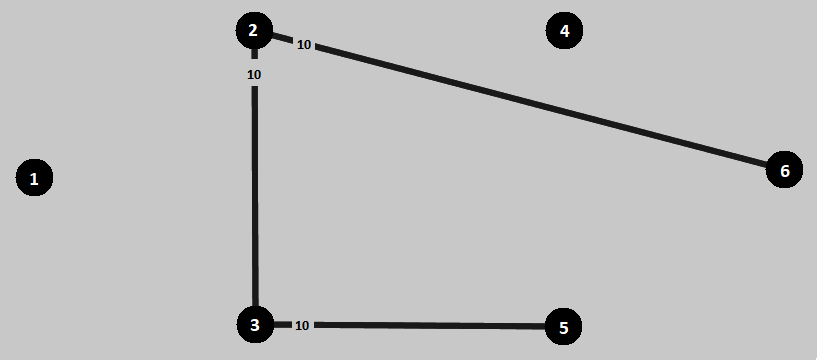
\includegraphics[width=13cm]{sdf/heuristic/transparent_protection/medium/logical_topology_odu3_medium}
\caption{ODU3 logical topology defined by the ODU3 traffic matrix.}
\label{logical_ODU3_protection_ref_medium_heuristic_transparent}
\end{figure}

\begin{figure}[H]
\centering
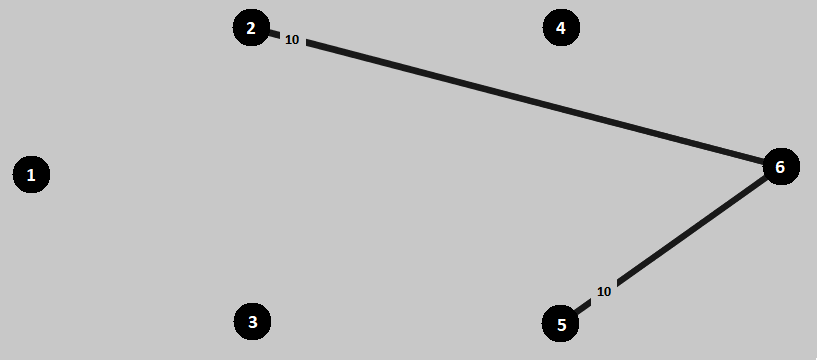
\includegraphics[width=13cm]{sdf/heuristic/transparent_protection/medium/logical_topology_odu4_medium}
\caption{ODU4 logical topology defined by the ODU4 traffic matrix.}
\label{logical_ODU4_protection_ref_medium_heuristic_transparent}
\end{figure}

\begin{figure}[H]
\centering
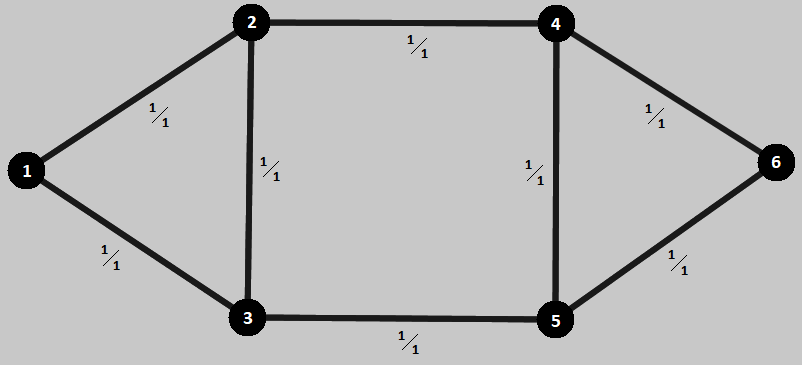
\includegraphics[width=13cm]{sdf/heuristic/transparent_protection/medium/physical_topology_medium}
\caption{Physical topology after dimensioning.}
\label{physical_topology_protection_ref_medium_heuristic_transparent}
\end{figure}

Following all the steps mentioned in the \ref{net2plan_guide}, applying the routing and grooming heuristic algorithms in the Net2Plan software and using all the data referring to this scenario, the obtained result for the Vasco's heuristics can be consulted in the following table \ref{scripttransp_protec_ref_medium_heuristic}.

\begin{table}[H]
\centering
\begin{tabular}{|| c | c | c | c | c | c | c ||}
 \hline
 \multicolumn{7}{|| c ||}{CAPEX of the Network} \\
 \hline
 \hline
 \multicolumn{3}{|| c |}{ } & Quantity & Unit Price & Cost & Total \\
 \hline
 \multirow{3}{*}{Link Cost} & \multicolumn{2}{ c |}{OLTs} & 16 & 15 000 \euro & 240 000 \euro & \multirow{3}{*}{283 520 000 \euro} \\ \cline{2-6}
 & \multicolumn{2}{ c |}{100 Gb/s Transceivers} & 566 & 5 000 \euro/Gb/s & 283 000 000 \euro & \\ \cline{2-6}
 & \multicolumn{2}{ c |}{Amplifiers} & 70 & 4 000 \euro & 280 000 \euro & \\
 \hline
 \multirow{10}{*}{Node Cost} & \multirow{7}{*}{Electrical} & EXCs & 6 & 10 000 \euro & 60 000 \euro & \multirow{10}{*}{59 990 900 \euro} \\ \cline{3-6}
 & & ODU0 Ports & 600 & 10 \euro & 6 000 \euro & \\ \cline{3-6}
 & & ODU1 Ports & 500 & 15 \euro & 7 500 \euro & \\ \cline{3-6}
 & & ODU2 Ports & 160 & 30 \euro & 4 800 \euro & \\ \cline{3-6}
 & & ODU3 Ports & 60 & 60 \euro & 3 600 \euro & \\ \cline{3-6}
 & & ODU4 Ports & 40 & 100 \euro & 4 000 \euro & \\ \cline{3-6}
 & & Line Ports & 566 & 1 000 \euro/Gb/s & 56 600 000 \euro & \\ \cline{3-6}
 & \multirow{3}{*}{Optical} & OXCs & 6 & 20 000 \euro & 120 000 \euro & \\ \cline{3-6}
 & & Line Ports & 1 132 & 2 500 \euro/porto & 2 830 000 \euro & \\ \cline{3-6}
 & & Add Ports & 142 & 2 500 \euro/porto & 355 000 \euro & \\
 \hline
 \multicolumn{6}{|| c |}{Total Network Cost} & 343 510 900 \euro \\
\hline
\end{tabular}
\caption{Table with detailed description of CAPEX of Vasco's 2016 results.}
\label{scripttransp_protec_ref_medium_heuristic}
\end{table}

\textbf{High Traffic Scenario:}\\

In this scenario we have to take into account the traffic calculated in \ref{high_traffic_scenario}. In a first phase we will show the various existing topologies of the network. The first are the allowed topologies, physical and optical topology, the second are the logical topology for all ODUs and finally the resulting physical and optical topology.\\

\begin{figure}[H]
\centering
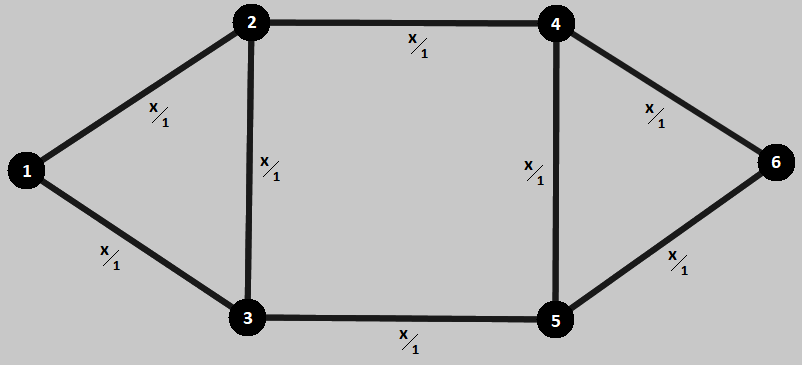
\includegraphics[width=13cm]{sdf/heuristic/transparent_protection/high/allowed_physical_high}
\caption{Allowed physical topology. The allowed physical topology is defined by the duct and sites in the field. It is assumed that each duct supports up to 1 bidirectional transmission system and each site supports up to 1 node.}
\label{allowed_physical_protection_ref_high_heuristic_transparent}
\end{figure}

\begin{figure}[H]
\centering
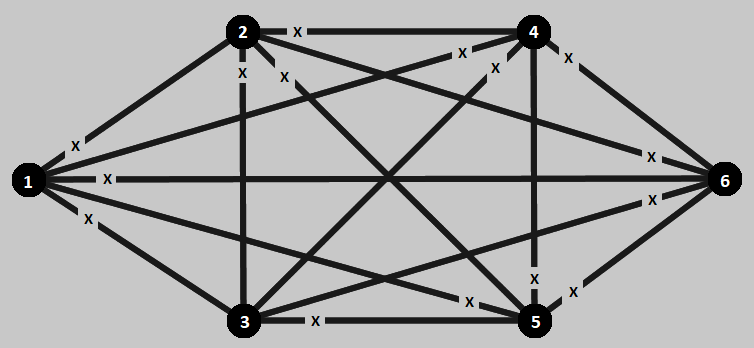
\includegraphics[width=13cm]{sdf/heuristic/transparent_protection/high/allowed_optical_high}
\caption{Allowed optical topology. The allowed optical topology is defined by the transport mode (transparent transport mode in this case). It is assumed that each connections between demands supports up to 100 lightpaths.}
\label{allowed_optical_protection_ref_high_heuristic_transparent}
\end{figure}

\begin{figure}[H]
\centering
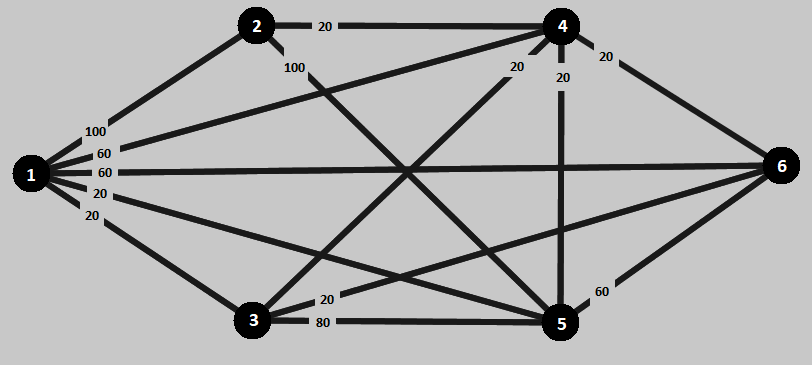
\includegraphics[width=13cm]{sdf/heuristic/transparent_protection/high/logical_topology_odu0_high}
\caption{ODU0 logical topology defined by the ODU0 traffic matrix.}
\label{logical_ODU0_protection_ref_high_heuristic_transparent}
\end{figure}

\begin{figure}[H]
\centering
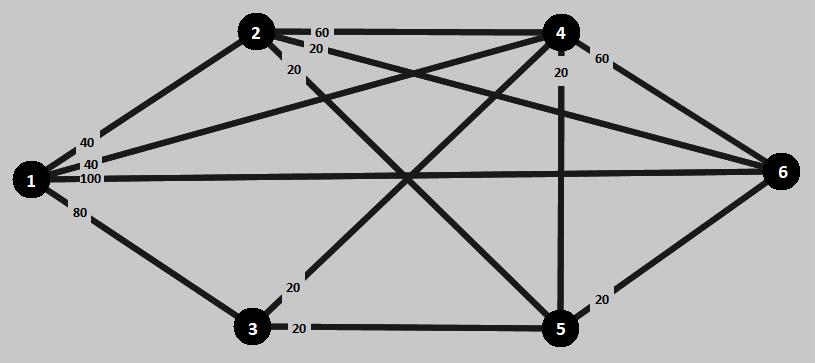
\includegraphics[width=13cm]{sdf/heuristic/transparent_protection/high/logical_topology_odu1_high}
\caption{ODU1 logical topology defined by the ODU1 traffic matrix.}
\label{logical_ODU1_protection_ref_high_heuristic_transparent}
\end{figure}

\begin{figure}[H]
\centering
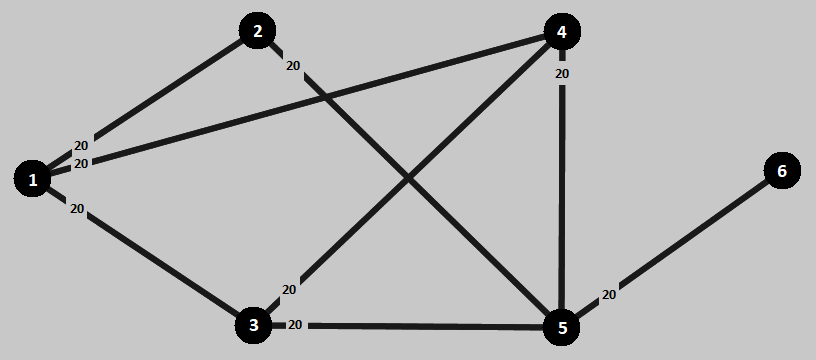
\includegraphics[width=13cm]{sdf/heuristic/transparent_protection/high/logical_topology_odu2_high}
\caption{ODU2 logical topology defined by the ODU2 traffic matrix.}
\label{logical_ODU2_protection_ref_high_heuristic_transparent}
\end{figure}

\begin{figure}[H]
\centering
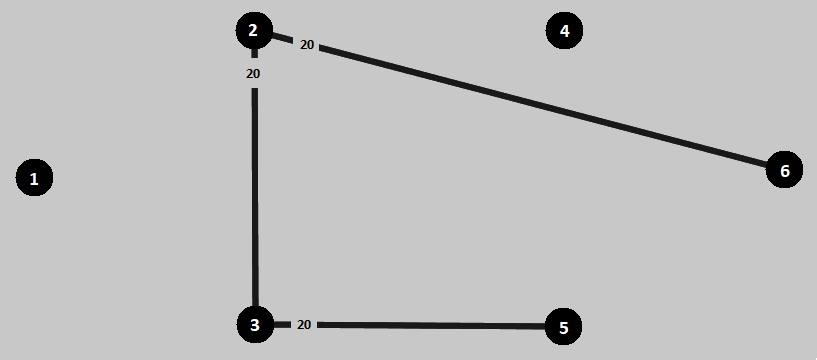
\includegraphics[width=13cm]{sdf/heuristic/transparent_protection/high/logical_topology_odu3_high}
\caption{ODU3 logical topology defined by the ODU3 traffic matrix.}
\label{logical_ODU3_protection_ref_high_heuristic_transparent}
\end{figure}

\begin{figure}[H]
\centering
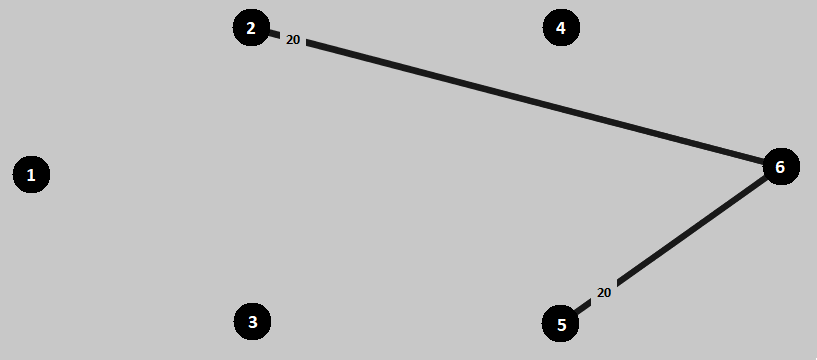
\includegraphics[width=13cm]{sdf/heuristic/transparent_protection/high/logical_topology_odu4_high}
\caption{ODU4 logical topology defined by the ODU4 traffic matrix.}
\label{logical_ODU4_protection_ref_high_heuristic_transparent}
\end{figure}

\begin{figure}[H]
\centering
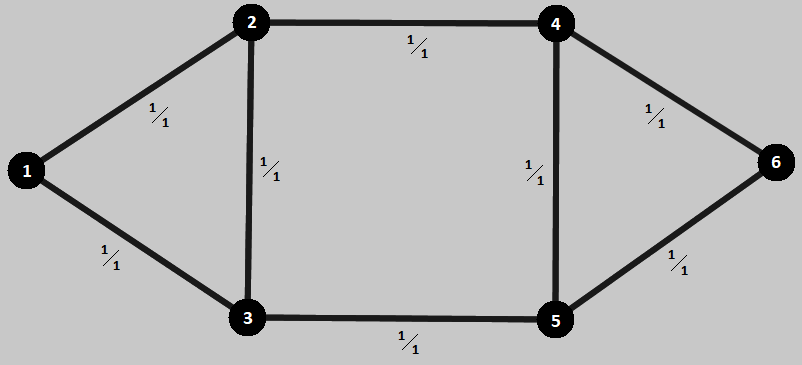
\includegraphics[width=13cm]{sdf/heuristic/transparent_protection/high/physical_topology_high}
\caption{Physical topology after dimensioning.}
\label{physical_topology_protection_ref_high_heuristic_transparent}
\end{figure}

Following all the steps mentioned in the \ref{net2plan_guide}, applying the routing and grooming heuristic algorithms in the Net2Plan software and using all the data referring to this scenario, the obtained result for the Vasco's heuristics can be consulted in the following table \ref{scripttransp_protec_ref_high_heuristic}.

\begin{table}[H]
\centering
\begin{tabular}{|| c | c | c | c | c | c | c ||}
 \hline
 \multicolumn{7}{|| c ||}{CAPEX of the Network} \\
 \hline
 \hline
 \multicolumn{3}{|| c |}{ } & Quantity & Unit Price & Cost & Total \\
 \hline
 \multirow{3}{*}{Link Cost} & \multicolumn{2}{ c |}{OLTs} & 16 & 15 000 \euro & 240 000 \euro & \multirow{3}{*}{530 520 000 \euro} \\ \cline{2-6}
 & \multicolumn{2}{ c |}{100 Gb/s Transceivers} & 1 060 & 5 000 \euro/Gb/s & 530 000 000 \euro & \\ \cline{2-6}
 & \multicolumn{2}{ c |}{Amplifiers} & 70 & 4 000 \euro & 280 000 \euro & \\
 \hline
 \multirow{10}{*}{Node Cost} & \multirow{7}{*}{Electrical} & EXCs & 6 & 10 000 \euro & 60 000 \euro & \multirow{10}{*}{112 201 800 \euro} \\ \cline{3-6}
  & & ODU0 Ports & 1 200 & 10 \euro & 12 000 \euro & \\ \cline{3-6}
 & & ODU1 Ports & 1 000 & 15 \euro & 15 000 \euro & \\ \cline{3-6}
 & & ODU2 Ports & 320 & 30 \euro & 9 600 \euro & \\ \cline{3-6}
 & & ODU3 Ports & 120 & 60 \euro & 7 200 \euro & \\ \cline{3-6}
 & & ODU4 Ports & 80 & 100 \euro & 8 000 \euro & \\ \cline{3-6}
 & & Line Ports & 1 060 & 1 000 \euro/Gb/s & 106 000 000 \euro & \\ \cline{3-6}
 & \multirow{3}{*}{Optical} & OXCs & 6 & 20 000 \euro & 120 000 \euro & \\ \cline{3-6}
 & & Line Ports & 2 120 & 2 500 \euro/porto & 5 300 000 \euro & \\ \cline{3-6}
 & & Add Ports & 268 & 2 500 \euro/porto & 670 000 \euro & \\
 \hline
 \multicolumn{6}{|| c |}{Total Network Cost} & 642 721 800 \euro \\
\hline
\end{tabular}
\caption{Table with detailed description of CAPEX of Vasco's 2016 results.}
\label{scripttransp_protec_ref_high_heuristic}
\end{table}

\vspace{15pt}

\subsubsection{Conclusions}

Once we have obtained the results for all the scenarios for transparent without survivability and transparent with 1+1 protection we will now draw some conclusions about these results. For a better analysis of the results will be created the table \ref{table_comparative_transparent_protec_heuristic} with the number of line ports, tributary ports and transceivers because they are important values for the cost of CAPEX, the cost of links, the cost of nodes and finally the cost of CAPEX.\\

\begin{table}[H]
\centering
\begin{tabular}{| c | c | c | c |}
 \hline
 & Low Traffic & Medium Traffic & High Traffic \\
 \hline\hline
 Traffic value & 0.5 Tbit/s & 5 Tbit/s & 10 Tbit/s \\ \hline
 Bidirectional Links used & 8 & 8 & 8 \\ \hline
 Number of Line ports & 136 & 566 & 1060 \\ \hline
 Number of Tributary ports & 136 & 1 360 & 2 720 \\ \hline
 Number of Transceivers & 136 & 566 & 1060 \\ \hline
 Link Cost & 68 520 000 \euro & 283 520 000 \euro & 530 520 000 \euro \\ \hline
 Node Cost & 14 547 590 \euro & 59 990 900 \euro & 112 201 800 \euro \\ \hline
 CAPEX without survivability & \textbf{32 247 590 \euro} & \textbf{128 130 900 \euro} & \textbf{238 581 800 \euro} \\ \hline
 CAPEX/bit without survivability & \textbf{64 495 180 \euro} & \textbf{25 626 180 \euro} & \textbf{23 858 180 \euro} \\
 \hline
 CAPEX with 1+1 protection & \textbf{83 067 590 \euro} & \textbf{343 510 900 \euro} & \textbf{642 721 800 \euro} \\ \hline
 CAPEX/bit with 1+1 protection & \textbf{166 135 180 \euro} & \textbf{68 702 180 \euro} & \textbf{64 272 180 \euro} \\
 \hline
\end{tabular}
\caption{Table with different value of CAPEX for this case.}
\label{table_comparative_transp_protec_heuristic}
\end{table}

Looking at the previous table we can make some comparisons between the transparent with 1+1 protection scenario:

\begin{itemize}
  \item Comparing the low traffic with the others we can see that despite having an increase of factor ten (medium traffic) and factor twenty (high traffic), the same increase does not occur in the final cost (it is lower);
  \subitem This happens because the number of the transceivers is lower than expected which leads by carrying the traffic with less network components and, consequently, the network CAPEX is lower;
  \item Comparing the medium traffic with the high traffic we can see that the increase of the factor is double and in the final cost this factor is very close but still inferior;
  \subitem This happens because the number of the transceivers is also lower but very close to the expected;
  \item Comparing the CAPEX cost per bit we can see that in the low traffic the cost is higher than the medium and high traffic, which in these two cases the value is very similar;
  \subitem This happens because the lower the traffic, the higher CAPEX/bit will be. We can see that in medium and high traffic the results tend to be one closer value.
\end{itemize}

We can also make some comparisons between the transparent without survivability and transparent with 1+1 protection scenarios:

\begin{itemize}
  \item We can see that in the transparent with 1+1 protection the CAPEX cost for all the three traffic is more than the double;
    \subitem This happens because in the transparent with 1+1 protection there is a need of having a primary and a backup path, in case of a network failure, and the backup path is typically longer and normally uses more than the double of the capacity of the primary;
  \item The number of the network components and the CAPEX cost are directly proportional to the traffic value. The higher the traffic value, the higher the network CAPEX cost;
  \subitem This happens because if the traffic value is higher, the network components have to be in more quantity to carry all the traffic end-to-end, both in the primary and backup paths;
  \item Comparing the CAPEX cost per bit we can see that has a similar case in both of the two scenarios. In the low traffic the cost is higher than the medium and high traffic, which in these two cases the value is very similar;
  \subitem This happens because the lower the traffic, the higher CAPEX/bit will be. We can see that in medium and high traffic the results tend to be one closer value.
\end{itemize} 